\documentclass{beamer}
\usepackage[utf8]{inputenc}
\usepackage[T1]{fontenc}

\usetheme{focus}
\definecolor{main}{RGB}{11, 93, 25}

\usecolortheme[RGB={11,93,20}]{structure}
\usepackage[spanish]{babel}

\usepackage{colortbl}
\usepackage{color}
\usepackage{pifont}
\usepackage{ulem}



\author{Alberto Molina Coballes}
\title{Intro a la virtualización}
\institute{IES Gonzalo Nazareno}
\titlegraphic{
\includegraphics[width=1.5cm]{cc_by_sa.png}}
\logo{
\includegraphics[width=.75cm]{logo_iesgn.png}}
\date{\today}

\usepackage{colortbl}
\usepackage{color}
\usepackage{pifont}
\definecolor{links}{HTML}{2A1B81}
\hypersetup{colorlinks,linkcolor=,urlcolor=links}
\definecolor{links}{HTML}{2A1B81}
%\hypersetup{urlcolor=links} % Does not apply color to href's
%\hypersetup{colorlinks,urlcolor=links} % href's are correct, but navigation lin%ks are magenta
\usepackage{tabularx}

\definecolor{verde}{rgb}{0,0.73,0}

\begin{document}
\begin{frame}[t,plain]
\titlepage
\end{frame}

\begin{frame}
  \begin{flushright}
    \textbf{(cc) 2011 Alberto Molina Coballes}\\
    Esta presentación se distribuye bajo licencia\\
    Creative Commons Reconocimiento 3.0 España.\\
    \url{http://creativecommons.org/licenses/by-sa/3.0/es/}\\
\vspace{1cm}
    Este documento incluye algunas partes de:\\
    \href{http://moodle.libresoft.es/pluginfile.php/131/mod_resource/content/6/virt1.pdf}{El arte de virtualizar}, de Miguel Vidal y José Castro.\\
  \end{flushright}
\end{frame}

\begin{frame}\frametitle{Índice}
\tableofcontents
% \begin{itemize}
% \item Virtualización
% \item Usos de Máquinas virtuales
% \item Ventajas e inconvenientes
% \item Principales técnicas de virtualización
% \item Virtualización completa
% \item Paravirtualización - I
% \item Paravirtualización - II
% \item Virtualización por hardware
% \item Comparativa
% \end{itemize}
\end{frame}

\section{Introducción}
\begin{frame}
  \frametitle{Virtualización}
    \begin{description}
    \item [Objetivo] Aumentar el rendimiento del hardware disponible
      incrementando el tiempo de procesamiento de un equipo, ya que
      habitualmente se desaprovecha gran parte.
    \item [Método] Instalar varios sistemas operativos en una misma
      máquina real para que funcionen como máquinas virtuales.
    \end{description}
\end{frame}

\begin{frame} \frametitle{¿Para qué se utiliza?}
  \begin{itemize}
  \item Consolidación de servidores
  \item Aislamiento e independencia de servicios y contenidos
  \item Laboratorio de pruebas
  \item Mantenimiento de sistemas antiguos
  \item Virtualización de arquitecturas de las que no se dispone
  \item Sistemas distribuidos
  \item Herramienta de aprendizaje
  \item Cloud computing
  \end{itemize}
\end{frame}

\begin{frame} \frametitle{Ventajas e inconvenientes}
  \begin{columns}
    \column{0.5\textwidth}
    \begin{description}
    \item [Principales ventajas]
    \end{description}
      \begin{itemize}
      \item Importante ahorro económico
      \item Seguridad
      \item Mayor aprovechamiento de recursos
      \item Migración en vivo
      \item Importante ahorro energético
      \end{itemize}
    \column{0.5\textwidth}
    \begin{description}
    \item[Principales inconvenientes]
    \end{description}
      \begin{itemize}
      \item Muchos sistemas dependen de un sólo equipo físico
      \item Penalizaciones en rendimiento
      \end{itemize}
  \end{columns}
\end{frame}

\subsection{Conceptos previos}
\begin{frame}
  \frametitle{Conceptos de virtualización}
  \begin{itemize}
  \item Al sistema operativo que ejecuta el software de virtualización
    se le conoce como anfitrión (\emph{host}).
    \begin{itemize}
    \item El anfitrión controla el hardware real.
    \end{itemize}
    \item Al sistema operativo virtualizado se le conoce como invitado
      o huésped (\emph{guest}).
      \begin{itemize}
      \item Puede haber varios huéspedes en un mismo anfitrión.
      \item Los huéspedes no deben interferir entre ellos ni con el
        anfitrión.
      \end{itemize}
  \end{itemize}
\end{frame}

\begin{frame}
  \frametitle{Conceptos de virtualización}
  \begin{itemize}
  \item Al software de virtualización se le llama:
    \begin{itemize}
    \item Hipervisor.
    \item Virtual Machine Manager (VMM).
    \end{itemize}
  \item El VMM o Hipervisor corre como parte del sistema operativo
    del anfitrión (o es el anfitrión)
  \item A una instancia del hardware virtualizado se la conoce
    como Máquina Virtual o VM.
  \item Los sistemas operativos huéspedes corren dentro de una
    VM. 
  \end{itemize}
\end{frame}

\begin{frame}
  \frametitle{Hipervisores (I)}
  \begin{itemize}
  \item Los hipervisores permiten que diferentes sistemas operativos,
    tareas y configuraciones de software coexistan en una misma
    máquina física.
  \item Abstraen los recursos físicos de la máquina anfitriona para las
    distintas máquinas virtuales.
  \item Garantizan un nivel de aislamiento entre los invitados.
  \item Proporcionan una interfaz única para el hardware.
  \end{itemize}
\end{frame}

\begin{frame}
  \frametitle{Hipervisores (y II)}
  Hay dos clases de hipervisores:
  \begin{description}
  \item [Tipo 1, nativo o \emph{bare-metal}] el hipervisor es una capa
    entre el hardware y el sistema operativo.
    \begin{itemize}
    \item Al sistema operativo se le llama Dominio de Control, Dominio
      Principal o Dom0 y corre sobre el hipervisor.
    \item Los huéspedes son Dominios Lógicos.
    \end{itemize}
    \item [Tipo 2 o \emph{hosted}] el hipervisor es una capa de
      software que corre sobre el sistema operativo anfitrión.
  \end{description}
\end{frame}

\begin{frame}[fragile]
  \frametitle{Extensiones de virtualización para x86}
  \begin{itemize}
  \item Desde 2005, Intel y AMD han añadido soporte hardware para la
    virtualización.
  \item Intel Virtualization Technology (VT) codename Vanderpool
  \item AMD Virtualization (AMD-V) codename Pacifica
  \item Añaden una funcionalidad específica para permitir a los
    hipervisores un rendimiento mayor en virtualización completa.
  \item La virtualización completa es más sencilla de implementar.
  \end{itemize}
  ¿Tiene estas extensiones mi CPU?
\begin{verbatim}
  egrep --color '(vmx|svm)' /proc/cpuinfo    
\end{verbatim}
\end{frame}

\section{Principales técnicas de virtualización}
\begin{frame} \frametitle{Principales técnicas de virtualización}
  \begin{description}
  \item[Emulación] La máquina virtual simula un hardware completo y el
    SO huésped sin modificar se ejecuta dentro de la VM.
  \item[Completa] El sistema operativo anfitrión simula
    el hardware (utilizando un \emph{hipervisor} tipo II) y sobre él se
    ejecutan los sistemas operativos huésped sin modificar
  \item[Por hardware o acelerada] Extensión de la virtualización
    completa, que es más eficiente al utilizar hardware (CPU) 
    adaptado.
  \item[Paravirtualización] Utiliza un \emph{hipervisor} tipo I sobre
    el que se ejecutan todos los dominios.
  \item[Contenedores o ligera] El SO está modificado para permitir múltiples
    procesos en diferentes espacios de usuario aislados unos de otros,
    cada uno con su configuración de red.
  \end{description}
\end{frame}

\subsection{Emulación}
\begin{frame} \frametitle{Emulación}
  \begin{columns}
    \column{0.5\textwidth}
    \begin{center}
    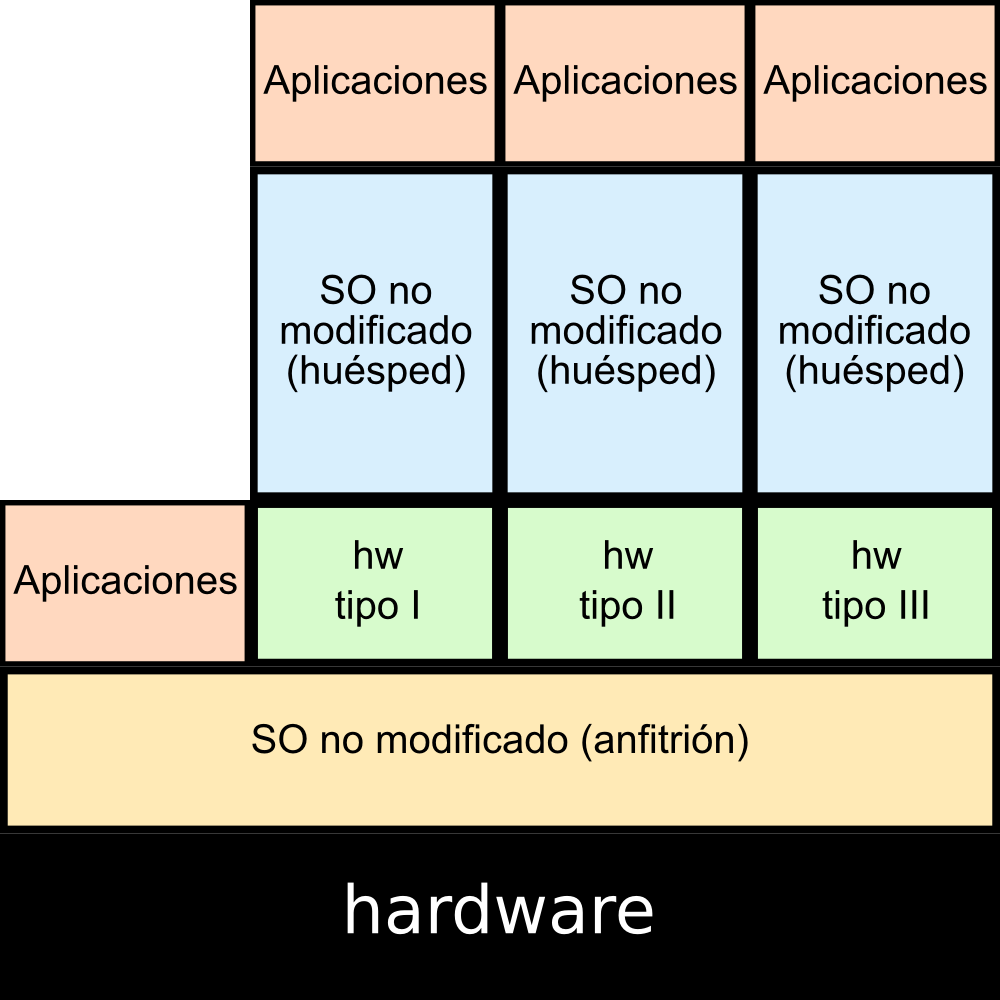
\includegraphics[width=0.9\textwidth]{img/emulacion.png}      
    \end{center}
    \column{0.5\textwidth}
    \begin{description}
    \item[Hardware] Convencional, además pueden emularse otras arquitecturas.
    \item[Ejemplos] Qemu
    \item [Ventaja] Facilidad de uso
    \item[Defecto] Bajo rendimiento
    \item[Utilización] Ejecutar sistemas sobre otras arquitecturas
      (e.g. ARM sobre x86)
    \end{description}
  \end{columns}
\end{frame}

\subsection{Virtualización completa}
\begin{frame} \frametitle{Virtualización completa}
  \begin{columns}
    \column{0.5\textwidth}
    \begin{center}
    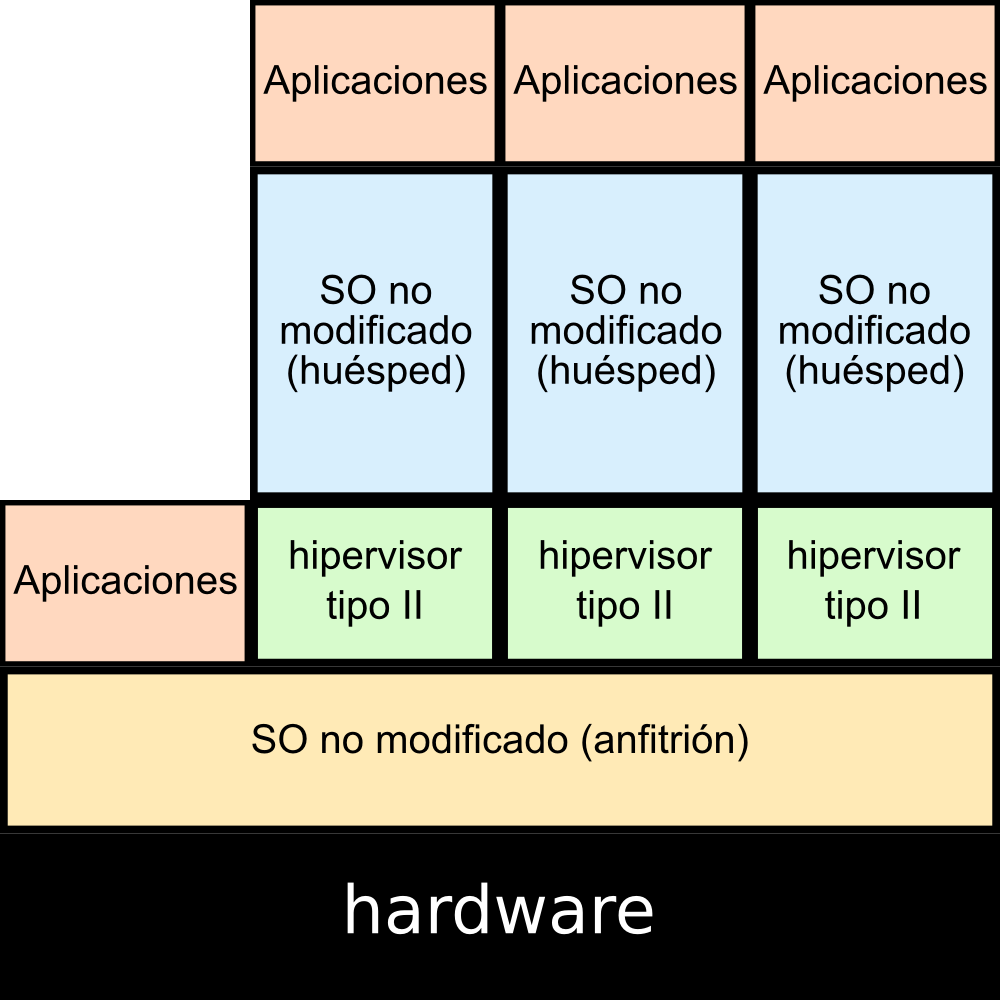
\includegraphics[width=0.9\textwidth]{img/virt_completa.png}      
    \end{center}
    \column{0.5\textwidth}
    \begin{description}
    \item[Hardware] Convencional
    \item[Hipervisor tipo II]
    \item[Ejemplos] VMWare Server, VirtualBox,
      Parallels Desktop, Virtual PC
    \item [Ventaja] Facilidad de uso
    \item[Defecto] Bajo rendimiento
    \item[Utilización] Virtualización en equipos convencionales
    \end{description}
  \end{columns}
\end{frame}

\subsection{Virtualización por hardware}
\begin{frame} \frametitle{Virtualización por hardware}
  \begin{columns}
    \column{0.5\textwidth}
    \begin{center}
    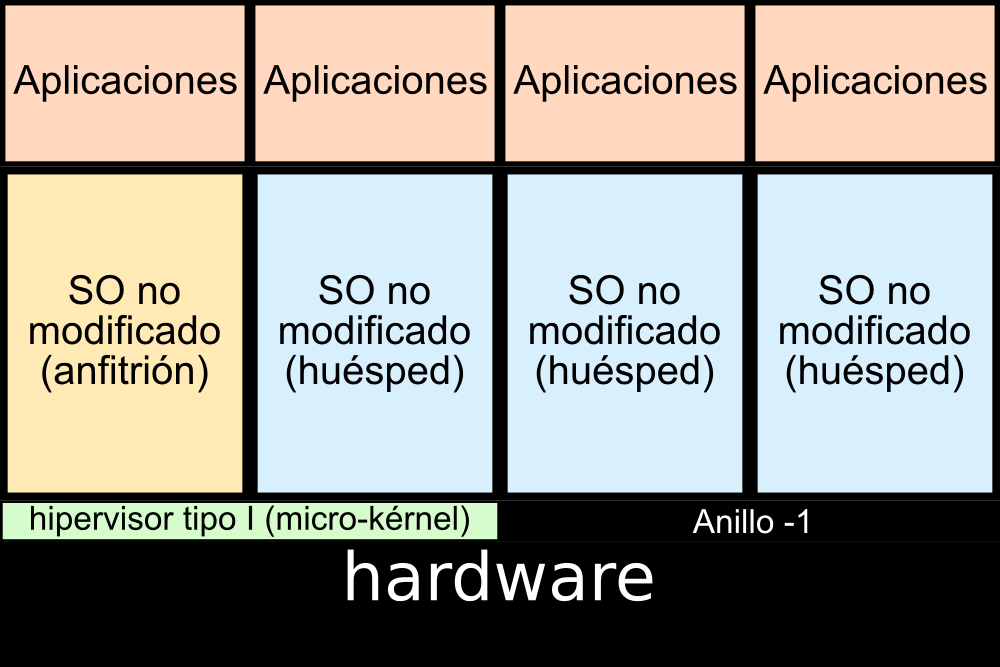
\includegraphics[width=0.9\textwidth]{img/virt_hw.png}      
    \end{center}
    \column{0.5\textwidth}
    \begin{description}
    \item[Hardware] Extensiones en CPU (Intel-VT, AMD-V)
    \item[Hipervisor tipo I]
    \item[Ejemplos] KVM, Xen HVM, Hyper-V
    \item [Ventajas] Alto rendimiento
    \item[Defecto] No sirve hw convencional
    \item[Utilización] Servidores/CPD
    \end{description}
  \end{columns}
\end{frame}

\subsection{Paravirtualización}
\begin{frame} \frametitle{Paravirtualización - I}
  \begin{columns}
    \column{0.5\textwidth}
    \begin{center}
    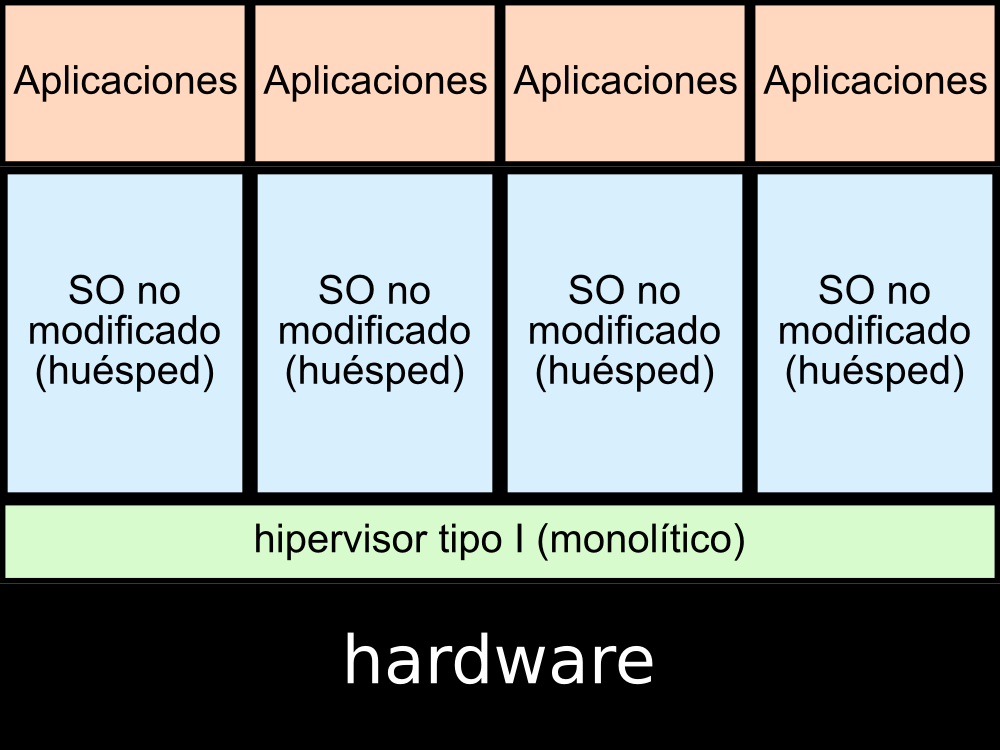
\includegraphics[width=0.9\textwidth]{img/paravirt_monolitica.png}      
    \end{center}
    \column{0.5\textwidth}
    \begin{description}
    \item[Hardware] Específico 
    \item[Hipervisor tipo I]
    \item[Ejemplos] VMware ESX(i)
    \item [Ventajas] SO huésped no modificado, alto rendimiento
    \item[Defecto] Poco hardware soportado
    \item[Utilización] Servidores/CPD
    \end{description}
  \end{columns}
\end{frame}

\begin{frame} \frametitle{Paravirtualización - II}
  \begin{columns}
    \column{0.5\textwidth}
    \begin{center}
    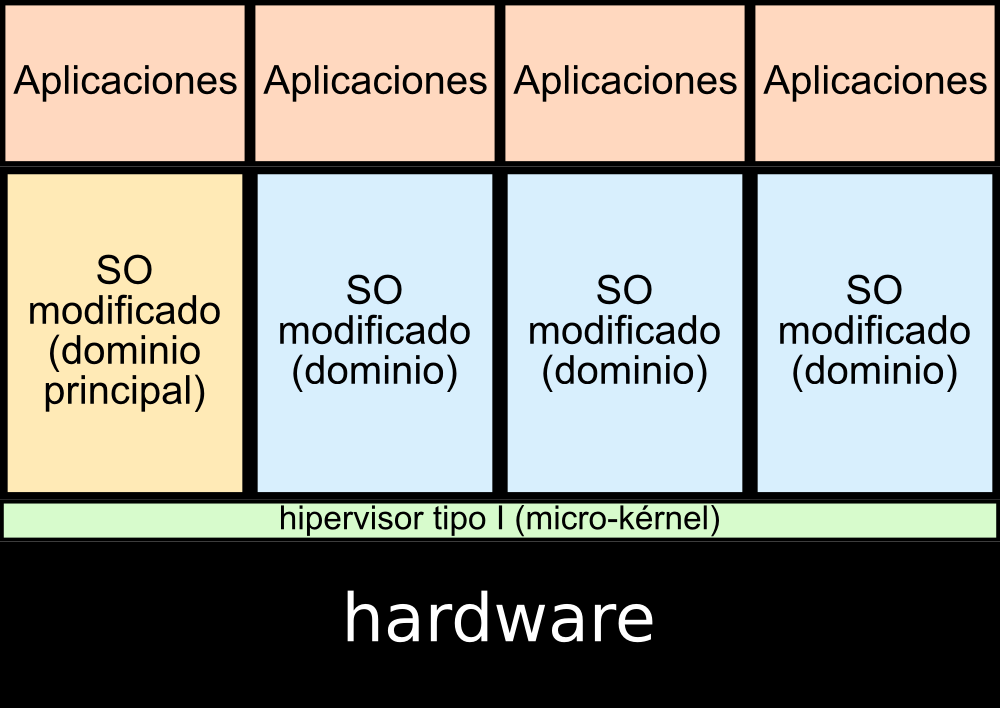
\includegraphics[width=0.9\textwidth]{img/paravirt_microkernel.png}      
    \end{center}
    \column{0.5\textwidth}
    \begin{description}
    \item[Hardware] Depende
    \item[Hipervisor tipo I]
    \item[Ejemplos] Xen, Hyper-V
    \item [Ventajas] Alto rendimiento
    \item[Defecto] SO modificado
    \item[Utilización] Servidores/CPD
    \end{description}
  \end{columns}
\end{frame}

\subsection{Virtualización ligera}
\begin{frame} \frametitle{Virtualización ligera o de Sistema Operativo}
  \begin{columns}
    \column{0.5\textwidth}
    \begin{center}
    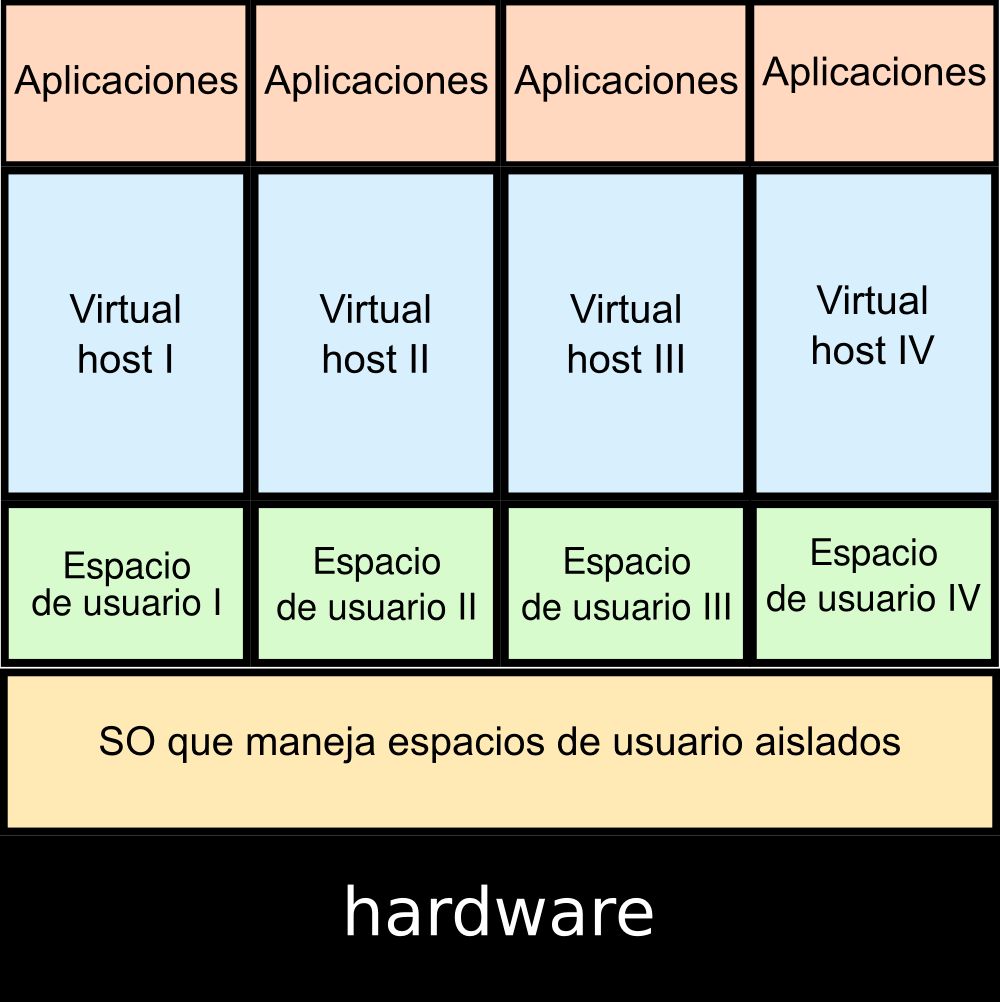
\includegraphics[width=0.9\textwidth]{img/virt_ligera.png}      
    \end{center}
    \column{0.5\textwidth}
    \begin{description}
    \item[Hardware] Convencional
    \item[Ejemplos] Jails, Containers, Virtuozzo, LXC, \ldots
    \item [Ventajas] Alto rendimiento, fácil implementación
    \item[Defecto] Aislamiento entre los virtual host, todos los SO iguales.
    \item[Utilización] Servidores/CPD
    \end{description}
  \end{columns}
\end{frame}

\subsection{Otros tipos de virtualización}
\begin{frame}
  \frametitle{Otros tipos de virtualización}
  \begin{itemize}
  \item Virtualización de bibliotecas: biblioteca Wine (subconjunto de
    la API de Win32 para poder ejecutar aplicaciones Windows)
  \item Virtualización de aplicación: entorno de ejecución virtual
    (con una API para la ejecución en diferentes
    plataformas). Ejemplo: Java Virtual Machine.
  \item Virtualización de escritorio: se implementa el escritorio como
    servicio. Ejemplo: SunVDI.
  \end{itemize}
\end{frame}

\section{Cuadro comparativo}
\begin{frame} \frametitle{Cuadro comparativo}
\noindent\begin{center}
    \begin{tabular}{|l|cccccc|}
      \hline
      Nombre & \multicolumn{5}{c}{Virtualización}& Licencia\\
      \cline{2-6}
      & Emu & Comp & Para & Hw & Cont & \\
      \hline
      \rowcolor[rgb]{1,0.95,0.77}
      Qemu & {\color{verde}\ding{51}}
      &{\color{red}\ding{55}}
      &{\color{red}\ding{55}}
      &{\color{red}\ding{55}}&{\color{red}\ding{55}} & Libre\\
      Xen &{\color{red}\ding{55}}      &{\color{red}\ding{55}}
      & {\color{verde}\ding{51}}
      &{\color{verde}\ding{51}} &{\color{red}\ding{55}}& Libre\\
      \rowcolor[rgb]{1,0.95,0.77}
      VirtualBox &{\color{red}\ding{55}}
      &  {\color{verde}\ding{51}}
      &{\color{red}\ding{55}}
      &{\color{red}\ding{55}}&{\color{red}\ding{55}} & Mixta\\
      LXC& {\color{red}\ding{55}}
      &{\color{red}\ding{55}}
      &{\color{red}\ding{55}}
      &{\color{red}\ding{55}}&{\color{verde}\ding{51}} & Libre\\
      \rowcolor[rgb]{1,0.95,0.77}
      Jails & {\color{red}\ding{55}}
      &{\color{red}\ding{55}}
      &{\color{red}\ding{55}}
      &{\color{red}\ding{55}}&{\color{verde}\ding{51}} & Libre\\
      Containers& {\color{red}\ding{55}}
      &{\color{red}\ding{55}}
      &{\color{red}\ding{55}}
      &{\color{red}\ding{55}}&{\color{verde}\ding{51}} & Libre\\
      \rowcolor[rgb]{1,0.95,0.77}
      KVM &{\color{red}\ding{55}}& {\color{red}\ding{55}}
      &{\color{red}\ding{55}}
      &{\color{verde}\ding{51}}&{\color{red}\ding{55}} & Libre \\
      VMWare ESX(i)& {\color{red}\ding{55}} & {\color{red}\ding{55}}
      & {\color{verde}\ding{51}}
      &{\color{red}\ding{55}}&{\color{red}\ding{55}} & Privativa \\ 
      Hyper-V & {\color{red}\ding{55}} &
      {\color{red}\ding{55}}& {\color{verde}\ding{51}} 
      &{\color{red}\ding{55}} &{\color{red}\ding{55}}& Privativa\\
      \rowcolor[rgb]{1,0.95,0.77}
      XenServer&{\color{red}\ding{55}}&
      {\color{red}\ding{55}} & {\color{verde}\ding{51}}
      &{\color{verde}\ding{51}} &{\color{red}\ding{55}}& Libre? \\
      Virtuozzo& {\color{red}\ding{55}} & {\color{red}\ding{55}}
      &{\color{red}\ding{55}}
      &{\color{red}\ding{55}}&{\color{verde}\ding{51}} & Privativa\\
      \hline
    \end{tabular}
  \end{center}
  \begin{flushright}
    \tiny{Fuente: \url{http://en.wikipedia.org/wiki/Comparison\_of\_platform\_virtual\_machines}}
  \end{flushright}
\end{frame}

\end{document}
